\section{Förderband}
Da die Schwungräder durch den Abwurf um ca. 40° (Yves fragen) abgebremst werden, müssen sie nach jedem Wurf erneut auf die gewünschte Drehzahl beschleunigt werden. Deshalb erfolgt die Zuführung der Bälle in getakteten Abständen. Ein weiteres Kriterium für eine konstante Wurfweite ist, dass die einzelnen Tennisbälle immer mit der gleichen Geschwindigkeit bei den Schwungrädern eintreffen. Die beste Art, beides zusammen zu realisieren ist ein Förderband. Das Förderband ist zwischen den zwei Acrylglasplatten aufgespannt. Der Antrieb des Förderbandes erfolgt mit einem DC-Motor welcher über ein ?eigenes Board ?angesteuert wird. Dieser ist mit einem Verhältnis von  5:1 untersetzt, um das benötigte Drehmoment an die Antriebswelle des Förderbandes zu übertragen. ?Die Berechnungen dazu sind im Anhang in Formel 28 ff. ersichtlich.? Die Antriebswelle und die Achse sind aus Aluminium gefertigt. Diese sind mittels Kugellager in den Seitenplatten gelagert. Die Antriebswelle, wo der Riemen angetrieben wird ist bombiert, damit dieser immer zentral auf der Welle liegt. Auf dem Förderband, welches aus einem Flachbandriemen besteht, sind konvexe Führungsschaufeln angebracht. Diese sind so ausgerundet, damit der Ball möglichst lange geführt werden kann und die Führungsschaufeln nicht in Berührung der Beschleunigungsrädern kommen. Die Schaufeln sind aus 1 mm dickem Aluminium Blech gefertigt. Dies konnte so nicht direkt beim Herteller bestellt werden, da diese im Herstellungsprozess nicht möglich war die Führungsschaufeln mittels der herkömmlichen Reibschweissmethode auf den Riemen aufzubringen. Deshalb wurden die Führungsschaufeln auf den Riemen aufgeklebt, welches sich auch als sehr gute Lösung zeigte. Aus diversen Testversuchen der Ballzuführung ist erkannt worden, dass für einen idealen Abwurf beide Räder zeitgleich den Ball beschleunigen müssen. Somit ist notwendig, dass die Bälle zunächst unterhalb des oberen Beschleunigungsrades gefördert und anschliessend in einem 45° Winkel nach oben zugeführt werden. Dazu dient ein Führungselement, welches auf beiden Seiten des Acrylglases angebracht ist. Dies sind der Form der Tennisbälle angepasst worden und mit dem 3D - Druck hergestellt worden.


\label{sec:Foerderband}
    Die Ansteuerung des Motors, der das Förderband antreibt erfolgt mittels PWM. Auf diese 
    weise lässt sich die Drehzahl und somit die Nachführgeschwindigkeit einstellen. Das 
    Band muss nur ein eine Richtung angetrieben werden, wodurch die Ansteuerung einfacher 
    realisiert werden kann. Das Schema ist in Abbildung \ref{abb:SchemaAnsteuerung} 
    ersichtlich. Im wesentlichen besteht diese Ansteuerung aus einem Vortreiber und eines 
    Schalters. Der Treiber dient dazu, den Schalter möglichst schnell und effizient zu 
    öffnen und zu schliessen. Auf diese Weise reduziert man die Schaltverluste. 
    \begin{figure}[h!]
    	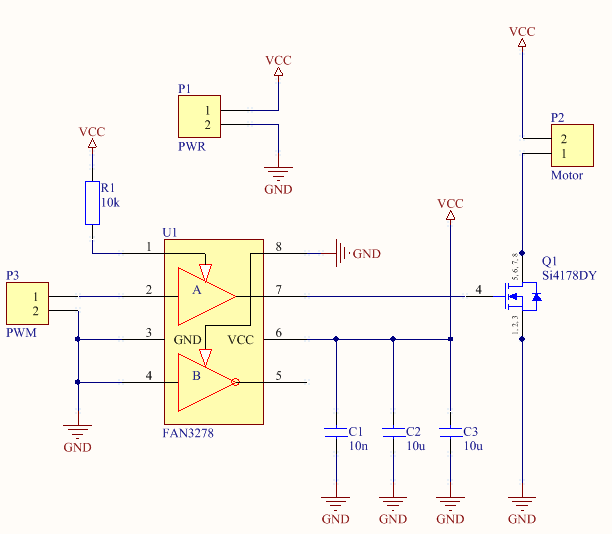
\includegraphics[width=0.4\textwidth,clip,trim=0mm 0mm 0mm 0mm]
    	{Enddokumentation/Bilder/Schema_DC-Ansteuerung.png}
    	\centering
    	\caption{Schema des Förderbandantriebes}
    	\label{abb:SchemaAnsteuerung}
    \end{figure}